\documentclass{article}
\usepackage[a4paper]{geometry}
\usepackage[utf8]{inputenc}

\usepackage{graphicx}
\graphicspath{ {./imatges_P3/imatges_informe/} }


\title{Informe pràctica 3\\Visió Artificial}
\author{Jordi Olivares Provencio\\Christian José Soler}

\begin{document}

\maketitle

\begin{enumerate}

 \item \textbf{Métodos de background substraction}

 \begin{enumerate}

 \item \textit{Encontrar  donde  se  acaba  una  escena  y  comienza  otra  (estos  frames  se denominan  shots del  vídeo).  ¿Qué  medida  de  las  imágenes  se  puede utilizar para distinguir las escenas?}
 
 A simple vista, no se pierden detalles, pero en el histograma se ve que hay diferencias sutiles entre las dos imágenes (original y reescalada).

 \item \textit{Aplicar  un  algoritmo  de  background  substraction  (consultar  el  material 
de teoría)}

 \item \textit{Visualizar, para  cada  segmento  delimitado  por  dos  shots  del  vídeo,  la  imagen 
estática extraída y las imágenes a partir de las cuales se ha obtenido}

 \item \textit{Comenta  en  detalle  la  implementación.  ¿Qué  sucede  si  los  shots  no  están 
correctamente  extraídos?    ¿Qué  sucede  si  encuentras  demasiados  shots  en  el 
vídeo?  Comenta qué representan  las  imágenes  estáticas  obtenidas.  ¿En  qué 
situaciones  el  algoritmo  funciona  y  en  cuáles  no? ¿Qué  sucede  si  restas  de  la 
imagen original la imagen del fondo? Visualízalo.}

 \item \textit{Ves  otras aplicaciones que se pueden sacar de este algoritmo?}

 \end{enumerate}

\newpage

 \item \textbf{Métodos de agrupación de datos numéricos}

 \begin{enumerate}
 \item \textit{La función gaussRandom (mu, sigma, numSamples), proporcionada con el 
enunciado,  permite  generar  nubes  de  puntos  con  una  distribución 
gaussiana con matriz de covarianza diagonal, utilizando como centro las 
coordenadas de mu. Genera tres nubes de 100 puntos con centros [1 2], [2 
2]  y  [2  1].  En  los  tres  casos  utilizar  una desviación  estándar  de  0.1  en 
todos los ejes. Visualiza los puntos generados (help: plot).}

 \item \textit{Utilizar el método kmeans para agrupar los datos anteriores. Visualizar en 
un mismo plot (help: subplot) una primera fila con los datos originales, y 
el  resultado  (incluyendo  los  centros)  de  las  agrupaciones  con  2,  3  y  4 
centros  respectivamente  en  la  segunda  fila  del  subplot,  utilizando 
diferentes colores (Figura 2).}

	La visualización del resultado de ambos apartados:
	
	\begin{center}
		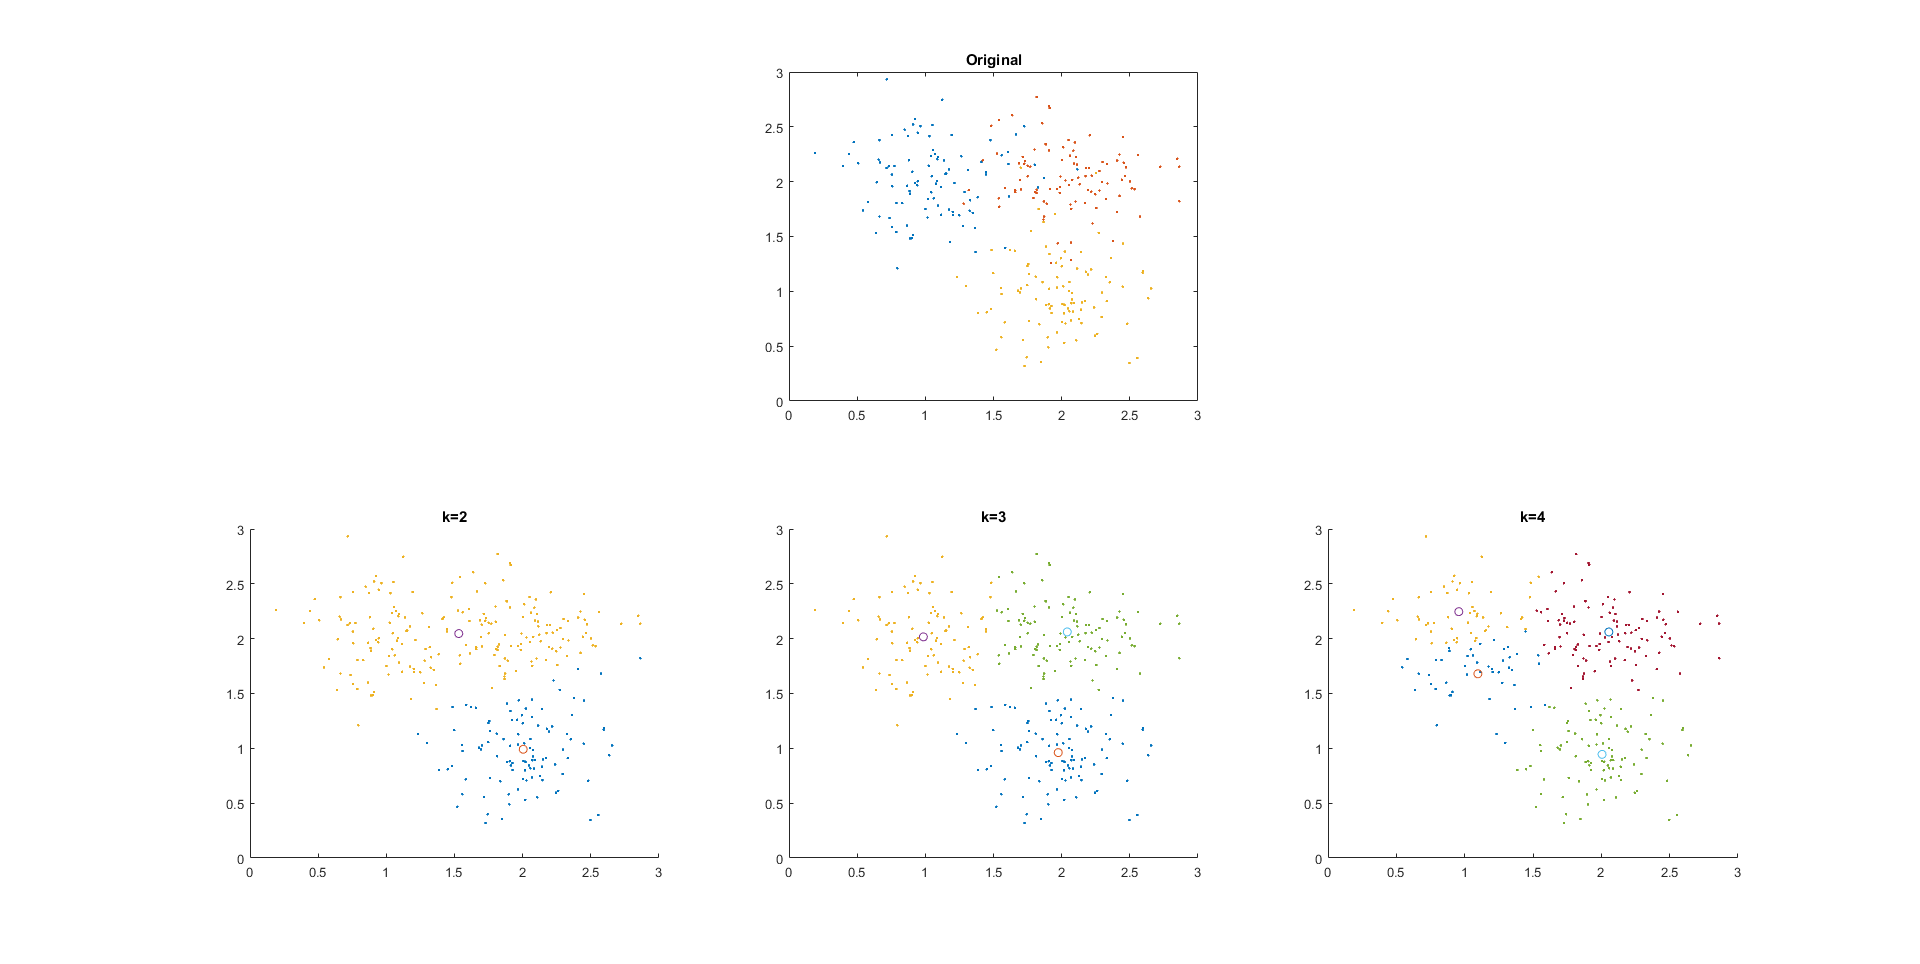
\includegraphics[width=\textwidth]{ej32-kmeans.png}
	\end{center}

 \item \textit{Comenta  los  resultados  que  has  encontrado,  valorando  el  número  de 
agrupaciones que has encontrado en cada caso y la similitud con los datos 
iniciales}
 
 Las agrupaciones reales se encontraron con $k=3$, ya que generamos los datos de manera que haya 3 grupos y se encontraron de forma satisfactoria. En el resto de casos, en k=2 hay 2 agrupaciones bastante claras y en $k=4$ según nuestra interpretación el clúster cuarto es bastante forzado, pero eso es consecuencia natural de kmeans, ya que este algoritmo encuentra tantas agrupaciones como $k$ le entremos.

 \end{enumerate}

\newpage

 \item \textbf{Métodos de agrupación: segmentación en el espacio RGB}

 \begin{enumerate}
 \item \textit{Lee  la  imagen   loro.png.  Conviértela  a  escala  de  grises  y  aplica  la 
segmentación  con  el  kmeans.  Prueba  diferentes  valores  de  k para 
encontrar la mejor segmentación.}

 \item \textit{Visualiza  la  imagen  segmentada  utilizando  el  nivel  de  gris  promedio 
encontrado con el método de segmentación. ¿A qué corresponde?}

 Como es un kmeans 2-dimensional, corresponde al centroide de cada clúster encontrado. A partir de aquí usamos el centroide para crear la segmentación de la imagen.

 \item \textit{Añade como características las coordenadas de los píxeles y comprueba si 
mejora el resultado de la segmentación}
  
	Resultado de comparativa para ver las diferencias entre hacer kmeans con posición y sin ellos (repitiendo el color 2 veces en este caso). El k-means es con $k=50$:
	
	\begin{center}
		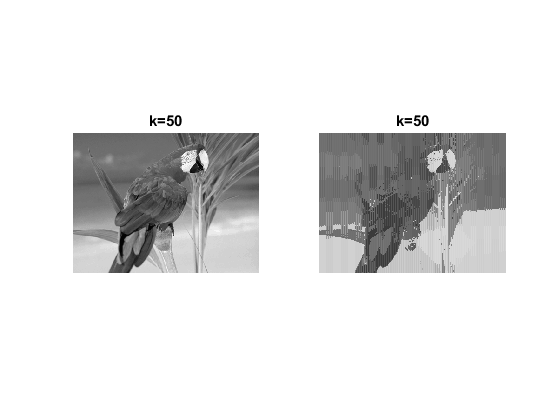
\includegraphics[width=0.8\textwidth]{ej33-loroGray.png}
	\end{center}
	
	Nos salen una rayas verticales dentro del k-means si añadimos la posición cosa que no sabemos exactamente porque nos pasa.
	
  \item \textit{A partir de la imagen de entrada, crea un matriz que contenga en cada fila la tripleta RGB de un píxel de la imagen. Tendrá tantas filas como píxeles 
haya en la imagen.}

 \item \textit{Utilizar el método kmeans para reducir el número de colores de la imagen 
a 16 colores diferentes.}
 
 \item \textit{Visualizar  en  una  misma  figura  las  imágenes  del  primer  apartado,  y  la imagen con 16 colores junto con su distribución de colores (Figura 3).}

	\begin{center}
		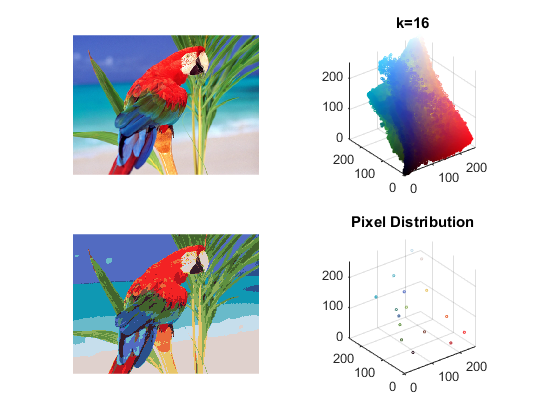
\includegraphics[width=0.8\textwidth]{ej33-loroRGB.png}
	\end{center}
 
 \end{enumerate}

\newpage

 \item \textbf{ Extracción de descriptores } 
 
 \begin{enumerate}
 \item \textit{¿A  qué  corresponden  las  variables f y  d que  devuelve  el método  vl\_sift? ¿Qué tamaño tienen? ¿A qué corresponden sus valores?}  
 
 $f$ contiene los frames resultantes del algoritmo SIFT, y $d$ contiene los descriptores de éstos. La primera tiene un tamaño de $4$ por el número de frames, y la segunda $128$ por el número de frames, en éste caso tenemos el número vale $282$.
 
 Los valores de $f$ en cada columna corresponden a $2$ elementos que indican el centro del frame, la escala de éste, y la orientación en radianes. Para $d$ tenemos que el vector de descripción són todos los histogramas de gradientes de los sub-patches juntos($8 \times 4 \times 4 = 128$)
 
 \item \textit{En  este  apartado  se muestran  los  puntos  característicos  detectados  con SIFT  en  una  misma  imagen  con  rotación.  Compara  los  resultados 
obtenidos antes y después de hacer la rotación y comenta lo que ves. ¿Hay 
invariancia a rotación? ¿Qué significa la línea que aparece en el interior de 
los círculos?}

\begin{center}
	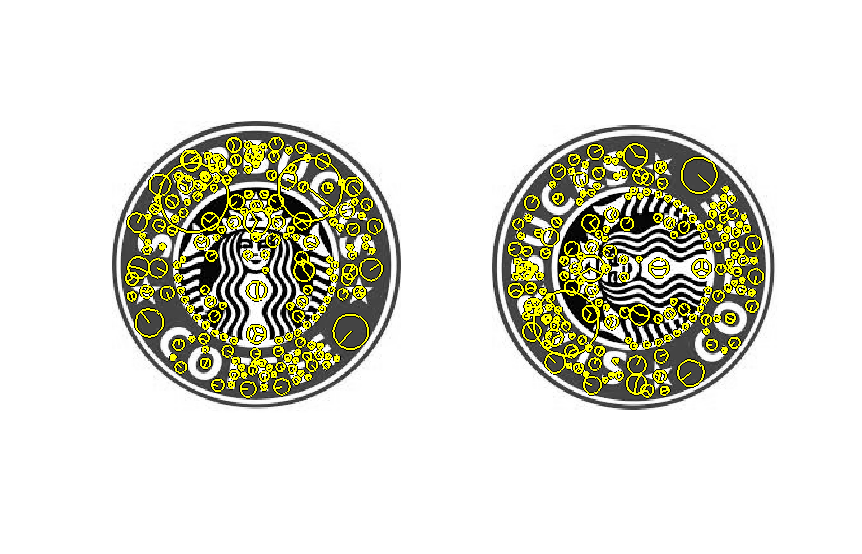
\includegraphics[width=0.8\textwidth]{ej34b.png}
\end{center}

Como podemos ver en la imagen, SIFT es invariante a la rotación. Vemos claramente que detecta los mismos puntos aunque girados. La línea que hay en medio indican la orientación del frame. Nos es útil para comparar los frames, ya que podemos normalizar con ellos la orientación de los frames.

 \item \textit{En  este  caso,  se  comparan  los  resultados  con  una  misma  imagen  a 
distintas  escalas.  Compara  los  resultados  obtenidos  antes  y  después  de 
hacer el reescalado y comenta lo que ves. ¿Hay invariancia a escala? ¿Qué 
significa el tamaño de los círculos que se muestran?}

\begin{center}
	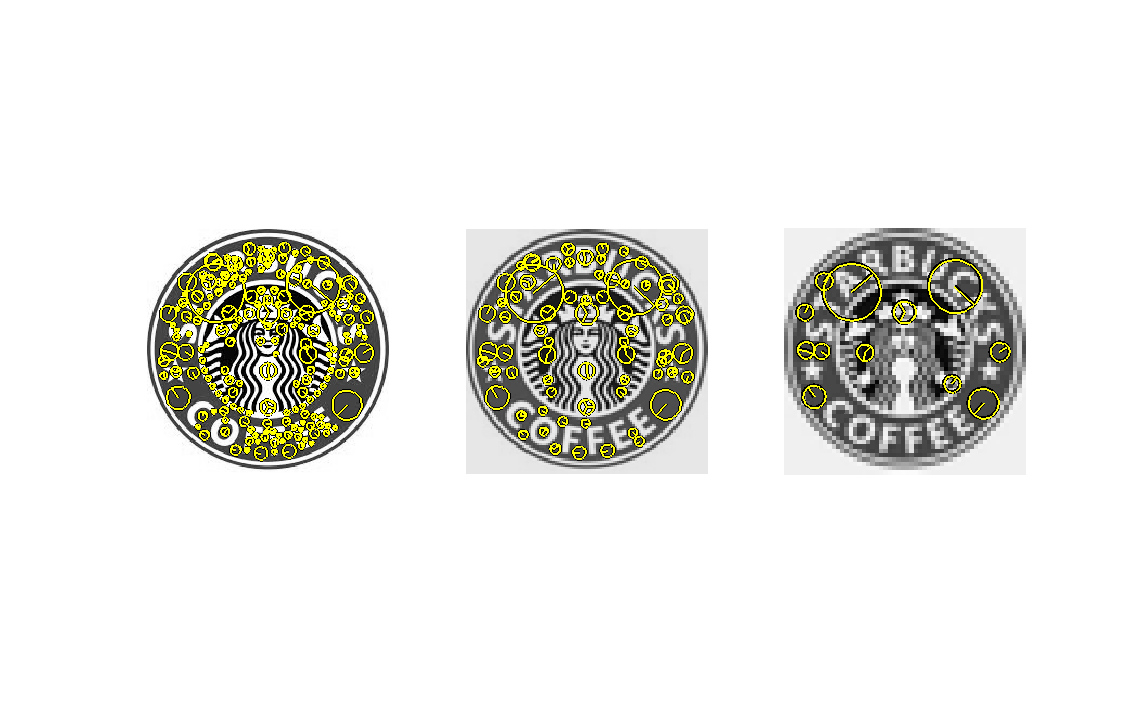
\includegraphics[width=0.8\textwidth]{ej34c.png}
\end{center}

En este caso vemos cómo el hacer un reescalado afecta a la hora de detectar los puntos con SIFT. En concreto, tenemos que nos impide calcular correctamente dónde hay esquinas en el paso del detector de Harris. El tamaño de los círculos indica el tamaño del frame, cuanto más grande más grande será el frame.

De hecho podemos ver que a medida que reescalamos la imagen, nos quedamos sólo con los frames más grandes ya que son los que sobreviven al reescalado.

 \item \textit{En este apartado se genera una imagen sintética y se calcula el descriptor 
en dos puntos distintos de la imagen.  Verás  que  se generan dos  figuras 
con el mismo  formato, pero con una pequeña diferencia en el cálculo del 
descriptor.  Fíjate  en los  descriptores  de la  fila inferior  del subplot.  ¿Qué 
diferencia  encuentras  entre  los  mostrados  en  la  primera  figura  y  la 
segunda?}

\begin{center}
	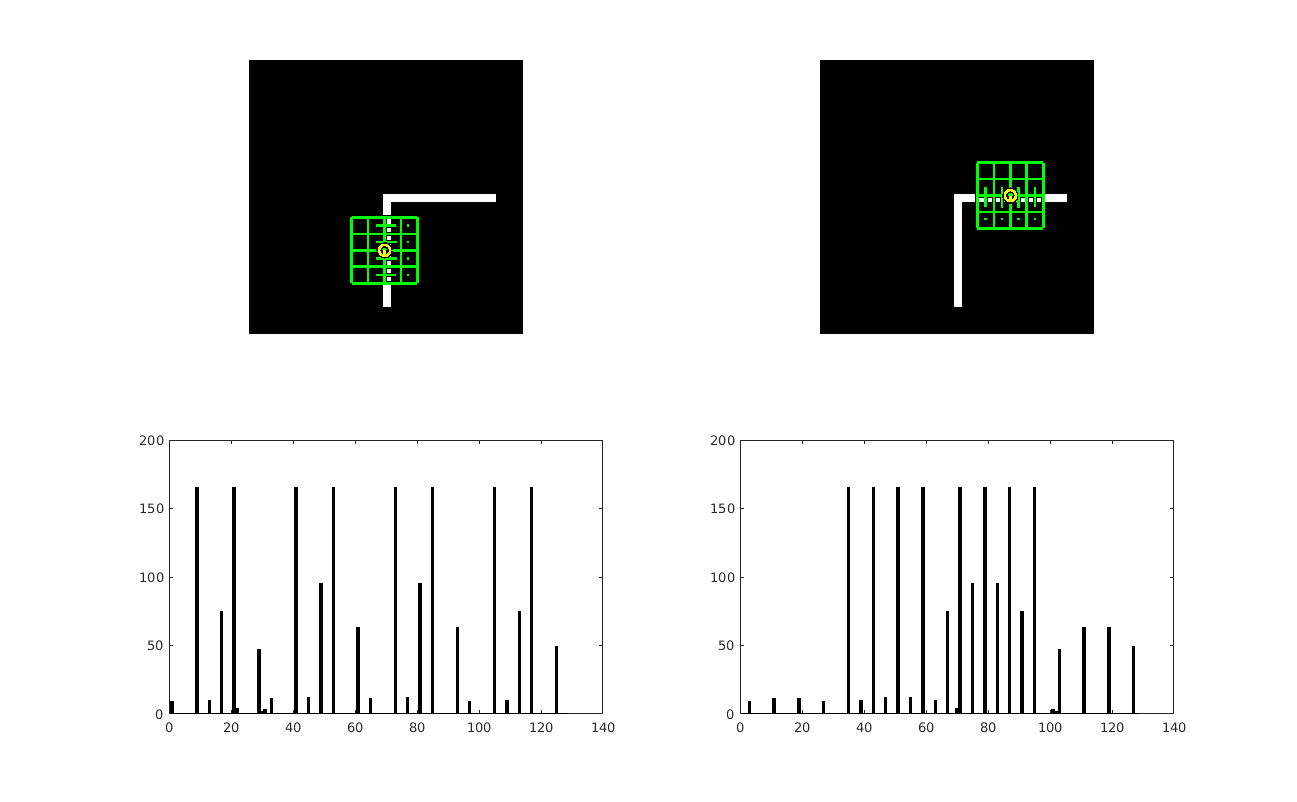
\includegraphics[width=0.8\textwidth]{ej34d1.png}
\end{center}

\begin{center}
	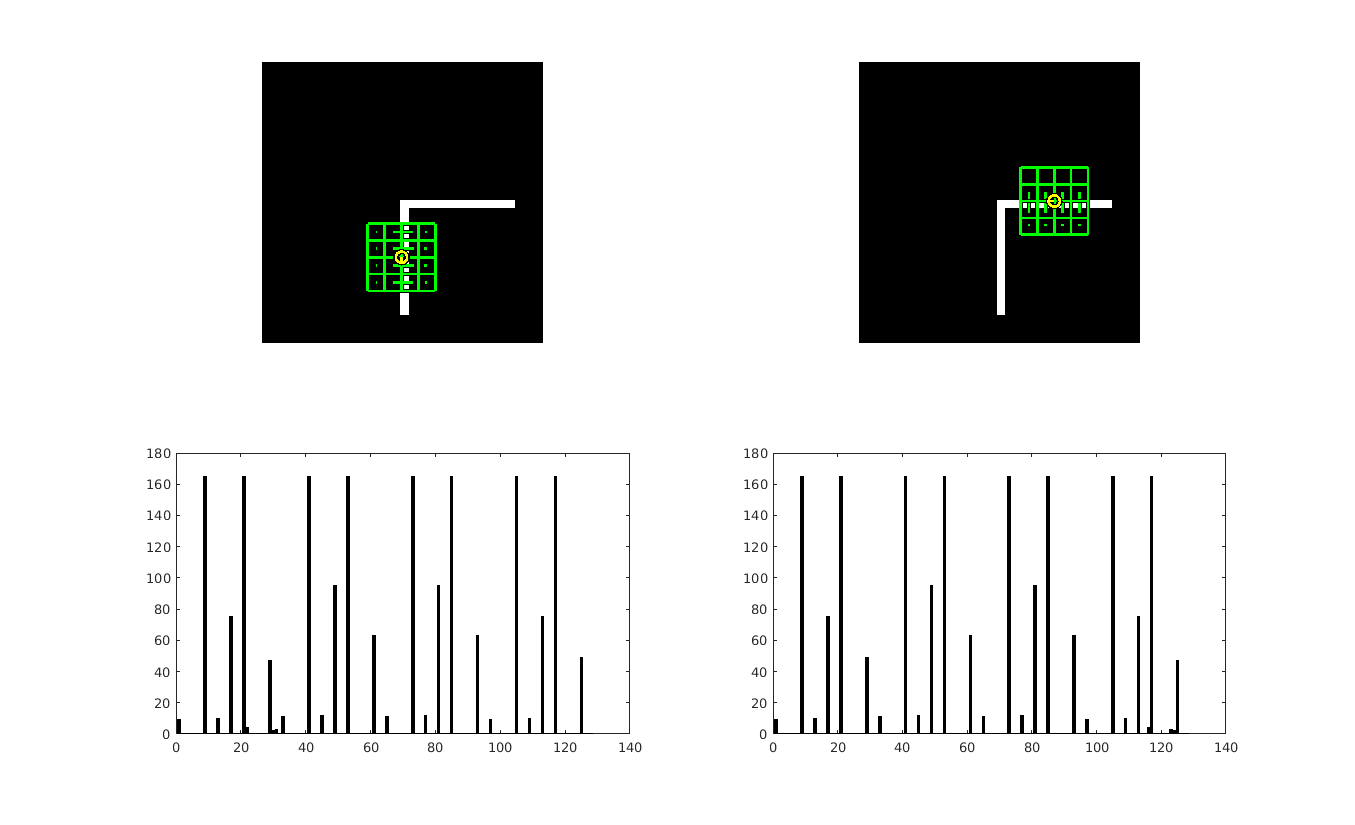
\includegraphics[width=0.8\textwidth]{ej34d2.png}
\end{center}

Vamos primero a comentar que la gráfica del descriptor se calcula teniendo en cuenta el frame. Además, la imagen sintética se genera con unos frames de SIFT proporcionados ya en el código. Éstos tienen ya la orientación indicada.

Ahora, la primera figura usa la orientación proporcionada en el frame, pero la segunda la calcula. De esta manera, a la hora de hacer la gráfica, como normalizamos los descriptores en base al frame y su orientación, los dos frames contienen la misma imagen con la orientación normalizada. Por tanto, tienen la misma gráfica de los descriptores.

 \end{enumerate}

\newpage

 \item \textbf{ Reconocimiento por alineación de puntos característicos}

 \begin{enumerate}
 \item \textit{Utiliza  el  método  showMatches usando  como  modelo  la  imagen 
 starbucks.jpg y como (nueva) escena la imagen starbucks6.jpg.}

 \item \textit{Repite el experimento  usando otras imágenes  como modelo  y/o escena. 
Para cada imagen modelo, enseña el  resto de imágenes de Starbucks en orden de su semejanza con el modelo.}

 \item \textit{¿Qué pasa si se le pasa una imagen que no contiene el logo de Starbucks? 
¿Qué  método  propondrías  (sin  implementarlo)  para  definir la 
probabilidad que la imagen “escena” corresponde a la imagen “modelo”?}

 \item \textit {Repite el experimento 4 veces cambiando las escalas y orientaciones del 
modelo. Comenta tus observaciones.}
 
 \end{enumerate}

\end{enumerate}

\end{document}
